
\chapter{UNH NASA MMS TableSat IA EXPERIMENTAL PLATFORM}
\label{chap:UNHTableSat1A}

The NASA MMS TableSat IA is a limited 3-DOF experimental test platform for the NASA MMS satellite (Figure \ref{fig:TSatFullView}).  The experimental platform is designed and constructed with the aid of other UNH Advanced Control Lab researchers to mimic the actual MMS spacecraft.  All electronics, booms, and actuators are attached to a circular PVC bus.  The aluminum hub at its center has a hollow center which allow it to rest on a center post giving the main platform full rotation about its z-axis and limited rotation about its x and y-axes.  Five out of the six booms present on the MMS spacecraft are represented on TableSat IA.  The four Spin-plane Double Probe (SDP) booms extend radially from the bus at 90 degree intervals.  One of the MMS's Axial Double Probe (ADP) booms is modeled with a boom attached to the center post of the TableSat.

\begin{figure}[H]
  \centerline{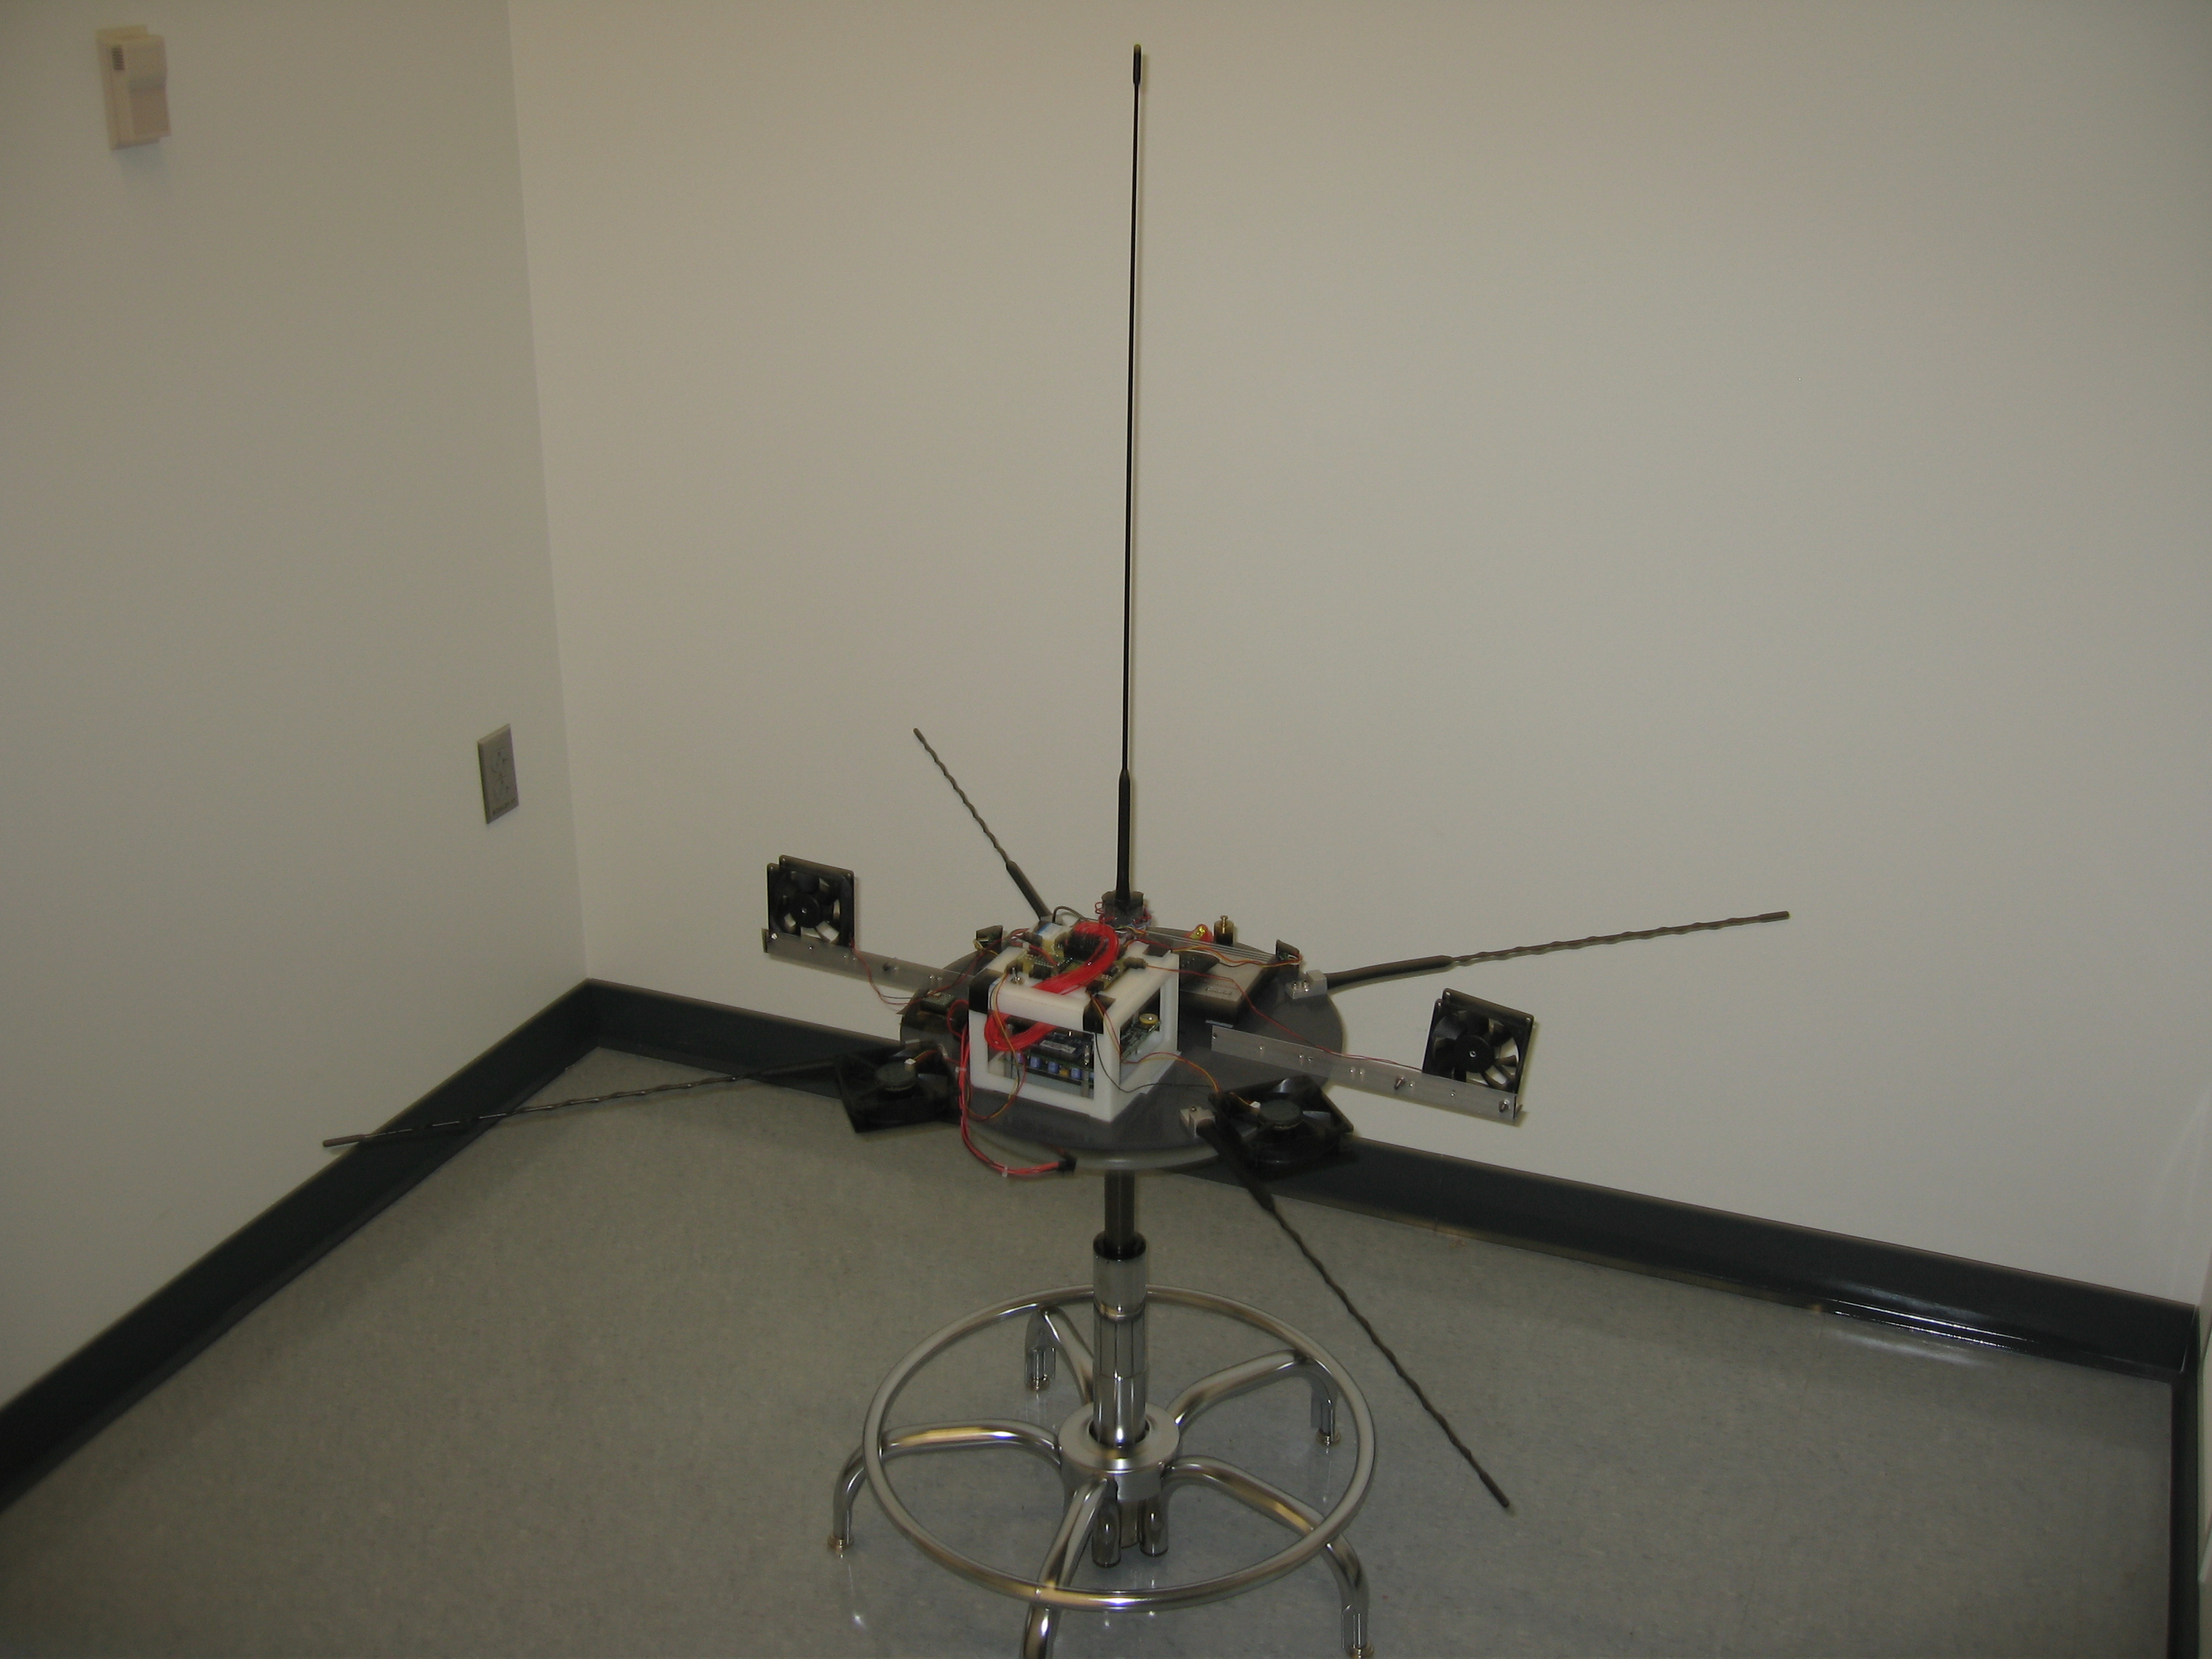
\psfig{file=figures/tsat_full_view.eps,height=3in}}
  \caption{TableSat IA Full View}
  \label{fig:TSatFullView}
\end{figure}

\section{Booms}
\label{sec:Booms}

The ADP booms are modeled with a selection of flexible antenna.  The physical model provides a basis for understanding the boom dynamics under rotation where the analytical tools in previous research \cite{mushawehthesis} were unable to.  Attaching weights to the tip and varying the stiffness of the selected antenna allows for some tuning to their fundamental frequency.  Since the SDP booms extend perpendicularly to gravity, two choices are made for their modeling.  For free motion, the cylindrical antenna for the ADP boom are also used for the SDP booms.  The disadvantage to these booms especially when adding weights to reduce their natural frequency is that they droop under the pull of gravity (Figure \ref{fig:WeightedSDPBooms}).  An alternative to the cylindrical antenna for the SPD booms are thin and flat strips of metal.  Attaching them to the TableSat's bus such that they are standing on edge removes the gravitational drooping, but still allows for the boom to bend back and forth in the spin plane.  This also restricts the boom's freedom of movement, so a combination of results is needed to predict the MMS boom's behavior while in orbit.


\begin{figure}[H]
  \centerline{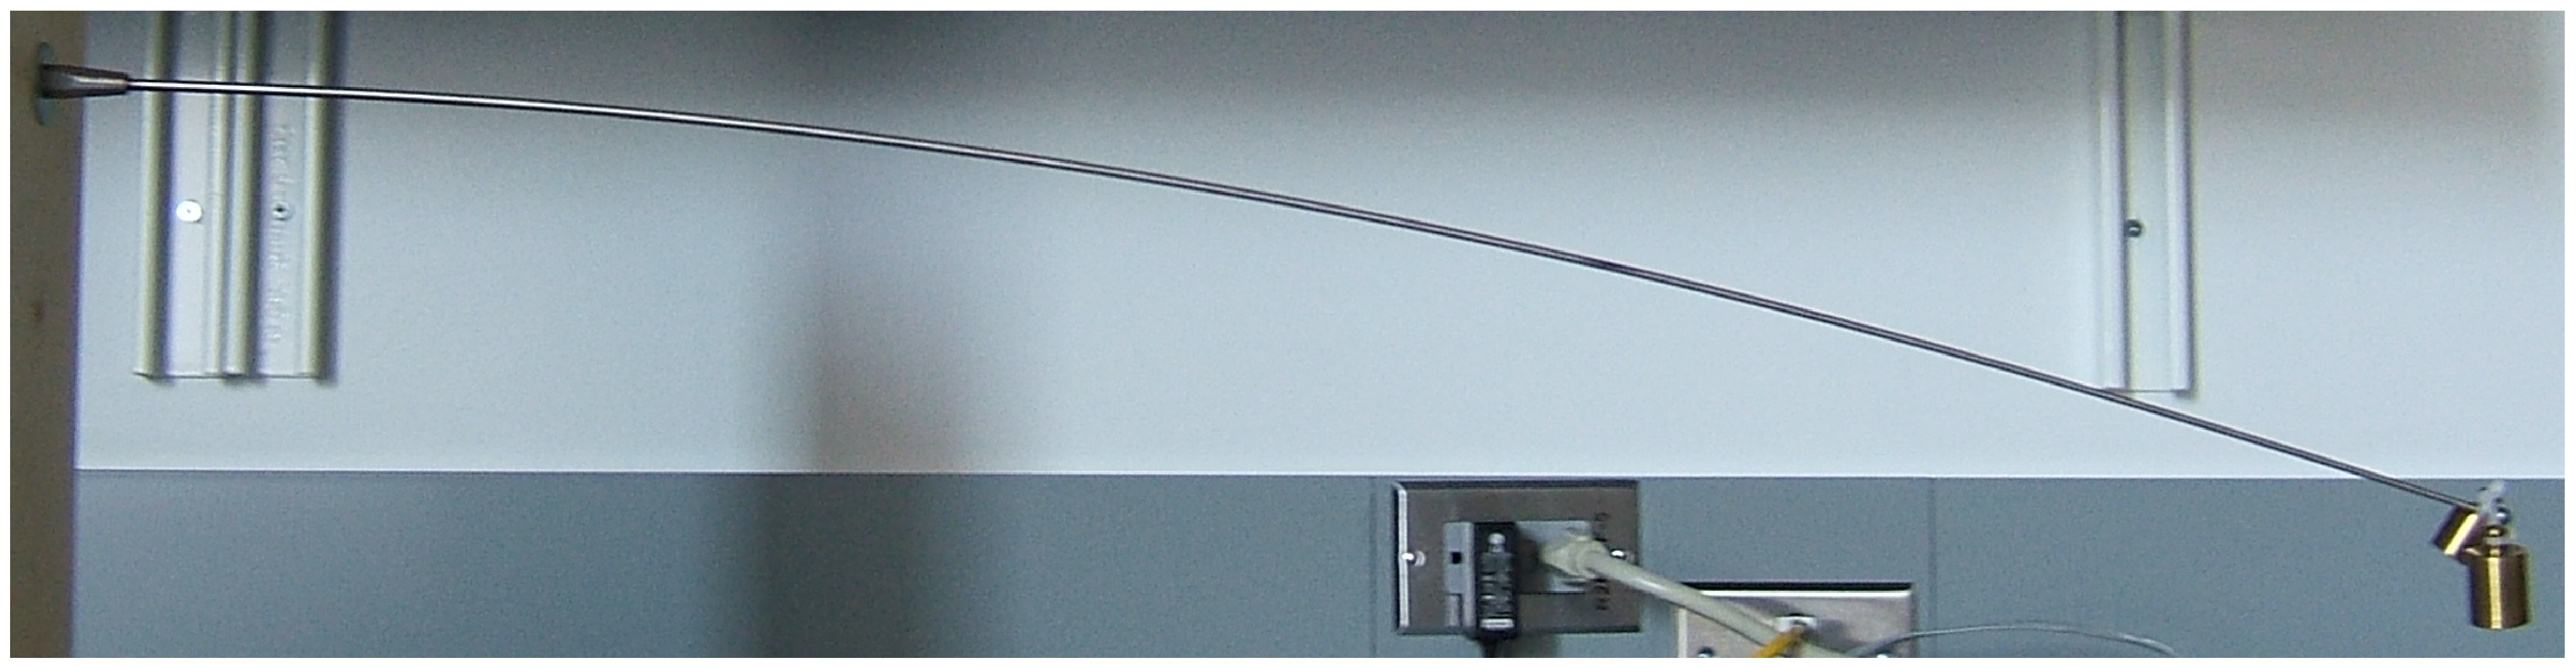
\psfig{file=figures/sdp_boom_droop.eps,width=6in}}
  \caption{Weighted SDP Booms \cite{laakso}}
  \label{fig:WeightedSDPBooms}
\end{figure}


\begin{figure}[H]
\centerline{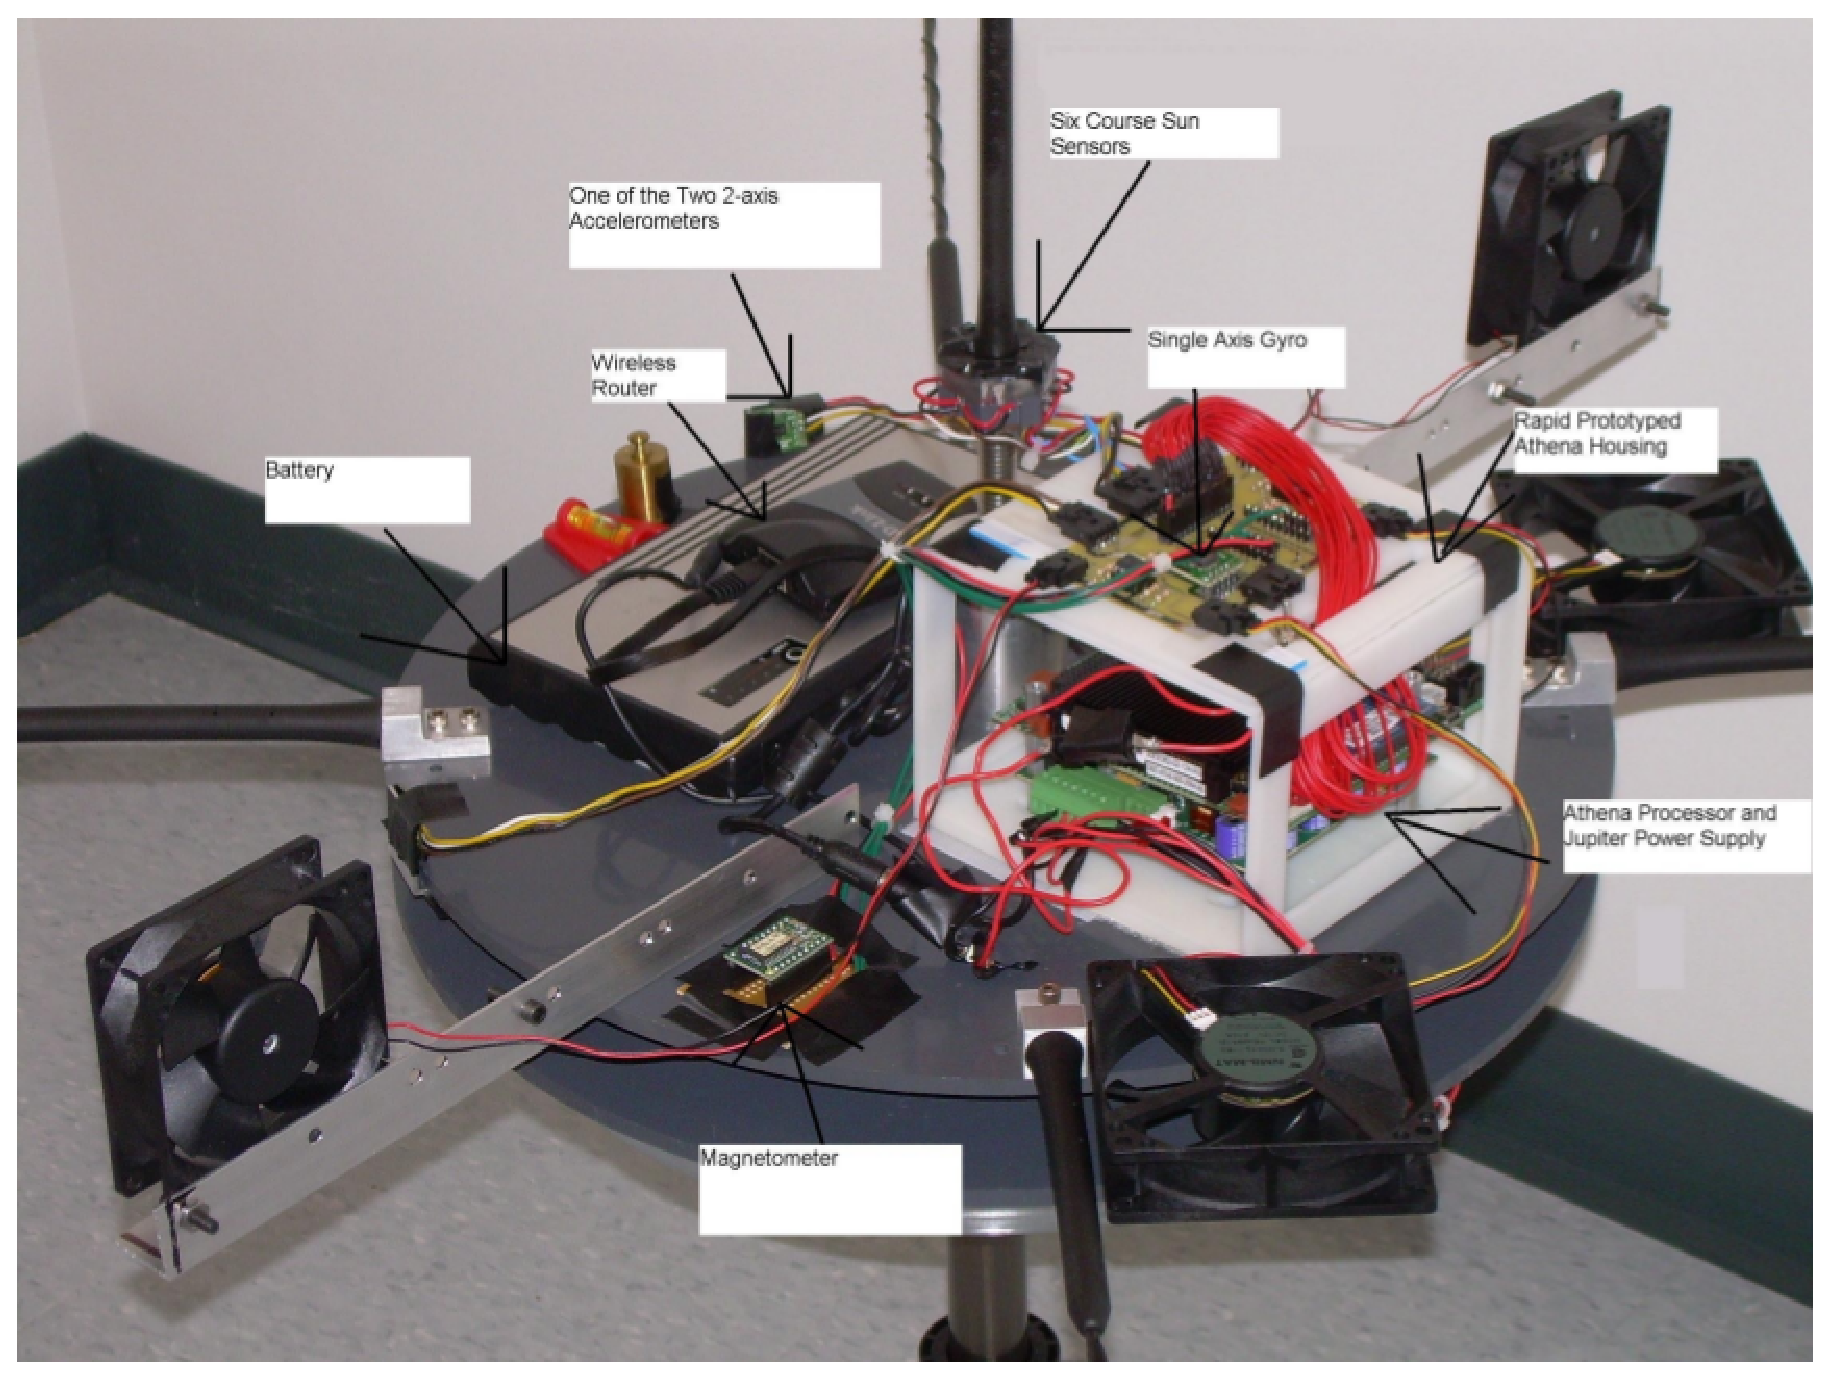
\psfig{file=figures/tsat_components.eps,height=4in}}
\caption{TableSat Components}
\label{fig:TSatComponents}
\end{figure}

\section{Flight Controller}
\label{sec:FlightController}

The on-board flight controller is an Athena PC from Diamond Systems powered by a Jupiter power supply and lithium-ion rechargeable battery.  The Athena processor and Jupiter power supply are mounted in a rapid prototyping housing with open sides for ventilation.  A custom printed circuit board (Figure \ref{fig:WiredPCB}), designed by members of the UNH TableSat IA team, is mounted on top of the rapid prototyping housing.  User Datagram Protocol (UDP) based communication (Section \ref{subsec:MessageDefinitions}) to the base station is transmitted through a wireless access point.

The UNH TableSat IA team also created a C program based off of Vess' ``open-loop'' flight controller \cite{vessthesis} .  This program is responsible for listening on a UDP socket on the TableSat and performing a limited set of actions based on the message packets it receives from the base station.  The most common messages triggered are actions such as altering the voltage commands to the actuators, scanning the sensor ports, and sending back the sensor voltage measurements to the base station through the UDP socket.

\begin{figure}[ht]
  \centerline{\psfig{file=figures/pcb_wired.eps,height=4in}}
  \caption{Wired Printed Circuit Board}
  \label{fig:WiredPCB}
\end{figure}


\section{Actuators}
\label{sec:Actuators}

In addition to the booms extending from the TableSat's bus, four single direction analog input computer fans are mounted to provide a source of thrust (Figure \ref{fig:TSatComponents}).  Two fans are mounted standing upright to provide radial torque and provide control to the rotation rate.  One pointing clockwise and the other counter clockwise have their centers level with the pivot point inside the central hub.  Two other fans are mounted facing down to provide limited opportunities for nutation control.  At a minimum, four single directional fans are needed to provide full state control for both positive and negative moments about the $x$ and $y$ axes.  The fans on TableSat IA provide limited thrust compared to the mass of the TableSat and friction in the mount point.  Through testing, the fans are found to provide insufficient thrust to differentiate between naturally damped out nutation from controlled nutation.  CO2 thrusters prove to be too powerful, freeze the solenoid valve, and lack the capacity to sustain the long thrusts needed for adequately controlled maneuvers.

\section{Sensors}
\label{sec:Sensors}

Four classes of analog sensors are implemented in NASA MMS TableSat IA's design: a gyroscope and accelerometer for velocity measurements and a coarse sun sensor and magnetometer for angular attitude measurements.  These sensors and the four actuators fill all available analog ports in the on-board Athena flight computer.

Figure \ref{fig:SensorVoltageReadings} shows the sensor reading as they are pulled into the base stations control system.  The top left plot contains the six voltage readings from the coarse sun sensors (CSS).  The CSS are easily saturated with ambient light as the sensor reading indicate in the plot.  A translucent film is added (Figure \ref{fig:CoarseSunSensorAssembly}) to address the saturated readings.  The top right portion of the graph contains the accelerometer readings.  AccelN1 and AccelN2 are 2g accelerometers and are oriented vertically at the edge of the bus to pick up accelerations due to nutation.  The AccelR1 and AccelR2 accelerometers are mounted at the edge of the bus as well but are oriented horizontally.  These sensors have a finer resolution at 0.5g since they do not need to compensate for the 1g of gravity.  The lower left plot shows the voltage produced by the single axis gyroscope, and the lower right contains the voltages for the three axes of the three-axis magnetometer.  With the gyroscope only available for validation and the AccelN1 and N2 with significantly high signal to noise ratios, that leaves the CSS, TAM, AccelR1, and R2 for attitude and angular velocity measurements.  After some additional testing it's found that the AccelR1 and R2 detect a mixture of changes to $\omega_z$ as well as a portion of the gravitational field as the sensor tilts slightly during a nutation.  This makes it difficult to differentiate a nutation from changes in angular velocity, so the TableSat's state measurement is left to the coarse sun sensor and magnetometer.

\begin{figure}[H]
  \centerline{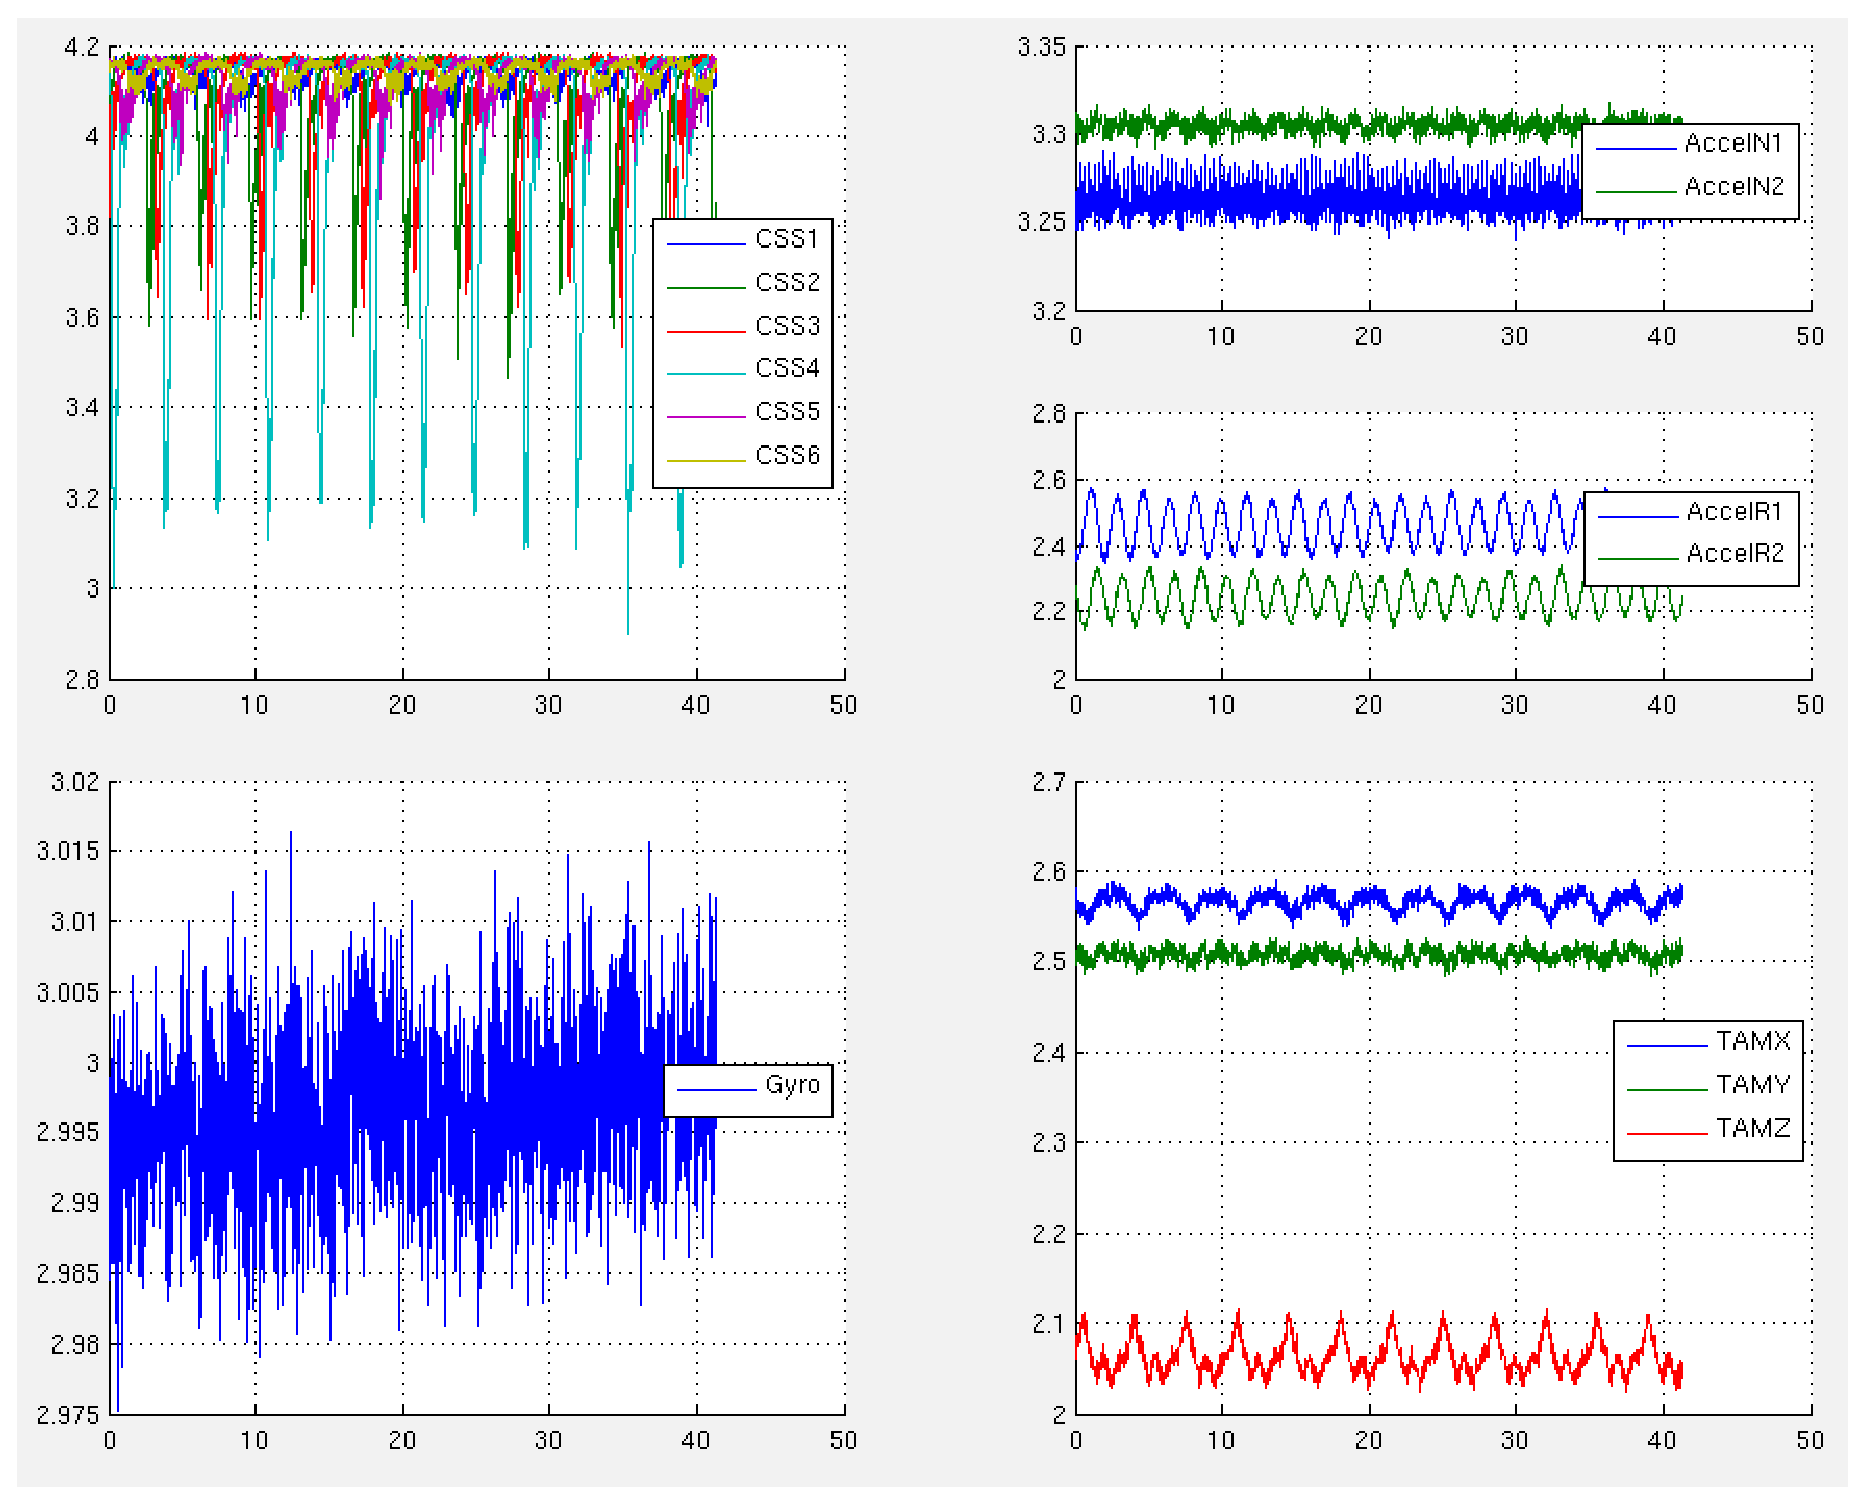
\psfig{file=figures/sensor_voltage_charts.eps,height=4in}}
  \caption{Sensor Voltage Readings}
  \label{fig:SensorVoltageReadings}
\end{figure}

Gyroscopes remain one of the most accurate sensors for detecting changes to a structure's angular body rates.  Unfortunately, they have significant weight and become unreliable at times.  Since any additional weight is a serious launch concern for a satellite, and because it has been shown that gyroless observer-based control of the MMS spacecraft is reliable \cite{mushawehthesis}, NASA has chosen to fly the MMS Mission without gyroscopes.  As such, this research uses the gyroscope solely as a verification method.  The gyroscope selected for TableSat IA is a single axis gyroscope that is mounted on a printed circuit board (Figure \ref{fig:WiredPCB}) at the top of the flight controller housing.  The gyroscope is oriented to detect changes in body rates about the TableSat's $z$ rotational axis.  It is mounted slightly above the center hub's pivot point and, therefore, unintentionally detects small signals from any limited nutation encountered.

Two 2-axis accelerometers are mounted at the outer circumference of TableSat's main bus.  The accelerometers are oriented such that one signal detects vertical acceleration with a 2g resolution and the other a radial signal with a 0.5g resolution.  It is observed that the rotational accelerometers also detect a small extraneous signal which is either due to oscillations in angular velocity or a nutation subjecting the radial accelerometer to gravitational effects.  The vertical components of the accelerometers operate with significantly low signal to noise ratio.  As a result, heavy filtering is required to even attempt to detect the out of plane rotations.  Any significant nutation allowed by the limited 3-DOF design are damped out quickly enough to be eliminated before the filtered accelerometer measurements is able to detect it.  Given these severe limitations in the sensor's measurements, it is decided to not incorporate the accelerometer measurements in this research.

The coarse sun sensors (CSS) used in the actual MMS spacecraft is represented on UNH TableSat IA as photodiodes mounted on a hexagonal piece of PVC pipe (Figure \ref{fig:CoarseSunSensorAssembly}).  Given that the gyroscope is used only for verification and not in the observer-based controller and that the accelerometers' noise levels make them impractical to use, the TableSat coarse sun sensors prove to be the most reliable sensor available.  It, however, is limited to measuring a single value, corresponding to rotations about the z-axis.  Photodiodes are light detectors that convert captured light to electricity.  Each photodiode detects light levels in its field of view and generates a voltage generally proportional to that value.  The photodiodes are mounted above the center hub and face outward from the axial center.  By placing a single light source in a dark room, the coarse sun sensors' voltages may be used to calculate the angular displacement about the body's z-axis.

\begin{figure}[ht]
  \centerline{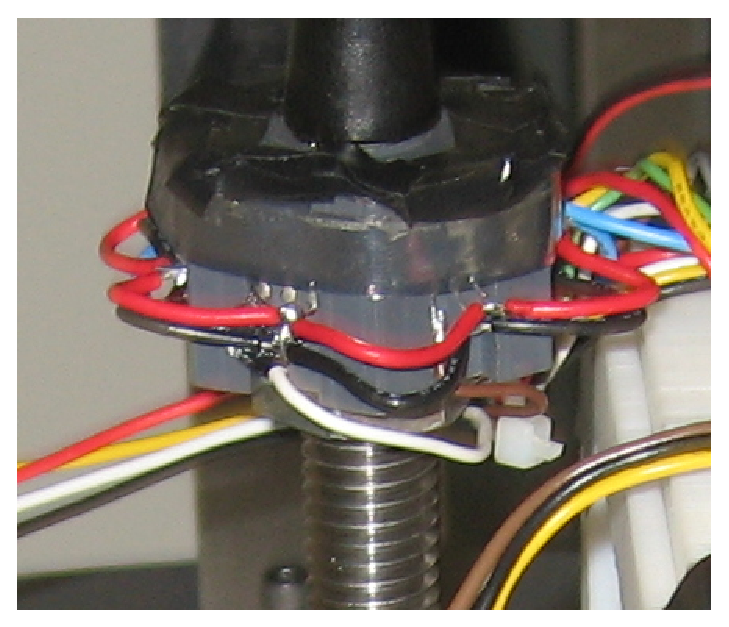
\psfig{file=figures/css_mounted.eps,height=2.5in}}
  \caption{Coarse Sun Sensor Assembly}
  \label{fig:CoarseSunSensorAssembly}
\end{figure}

Along with the coarse sun sensor, the three-axis magnetometer (TAM) is used to measure attitude.  The primary advantage of the TAM over the coarse sun sensor it that it provides the full attitude measurement rather than just z-axis rotation.  As seen in Figure \ref{fig:SensorVoltageReadings}, three voltages are reported to designate the TableSat's attitude.  Each of the three voltage outputs corresponds to the strength of the magnetic field in each respective orthogonal direction.

\chapter{SENSOR MEASUREMENTS}
\label{chap:SensorMeasurements}

\section{Coarse Sun Sensor Measurements}

Calculating the angular displacement about the body's z-axis is accomplished using a method similar to a resultant force calculation.  Assuming all of the photodiodes volts per lumen rates are consistent, the measured voltages can be described as an equivalent force in the direction of the photodiode face.  Each force is decomposed into its respective x and y components and then summed into a resultant force vector whose angle is used to represent the angular displacement of the TableSat.  Even though this method is fairly simplistic and that individual sensor voltage readings contains a moderate level of noise, this method is proven to generate a reliable and clean signal even before even incorporating filtering and estimation techniques.  Heading $\psi$ is calculated as follows:
\begin{subequations}
  \begin{align}
    V_{css\_x} & = \sum\limits_{i=1}^6 (V_{css\_i} - V_{css\_base}) \cos \left( \frac{2\pi}{6} (i-1)\right) \\
    V_{css\_y} & = \sum\limits_{i=1}^6 (V_{css\_i} - V_{css\_base}) \sin \left( \frac{2\pi}{6} (i-1)\right) \\
    \psi & = \tan^{-1} \frac{V_{css\_y}}{V_{css\_x}}
  \end{align}
  \label{eqn:CSSResultantForce}
\end{subequations}
Where $V_{css\_base}$ is the baseline voltage measurement for the coarse sun sensors, and $V_{css\_i}$ is the voltage reading for the $i$th photo diode.


\begin{figure}[H]
\centerline{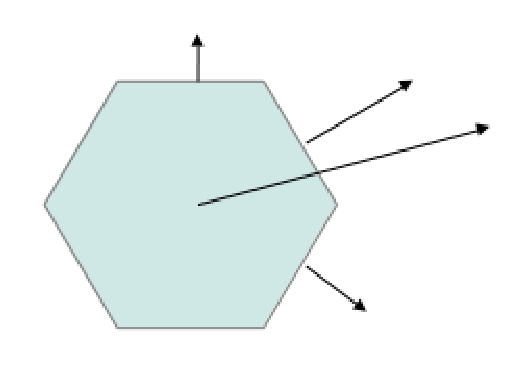
\psfig{file=figures/css_vectors.eps,height=1in}}
\caption{Photodiode Resultant Force Calculation for Yaw}
\label{fig:CSSVectors}
\end{figure}

\section{Three-Axis Magnetometer}
\label{sec:TheeAxisMagnetometer}

To determine a method of converting raw TAM voltages to a TableSat, the clockwise actuator is set to provide a constant thrust.  With the fraction of the pivot point, the system slowly stabilizes to a relatively constant spin rate.  Once stabilized, TAM voltage readings are recorded at a rate of 50 Hz and written to a log.  The mean values are subtracted from each of the three axes and plotted (Figure \ref{fig:TAMRaw}).

\begin{figure}[H]
\centerline{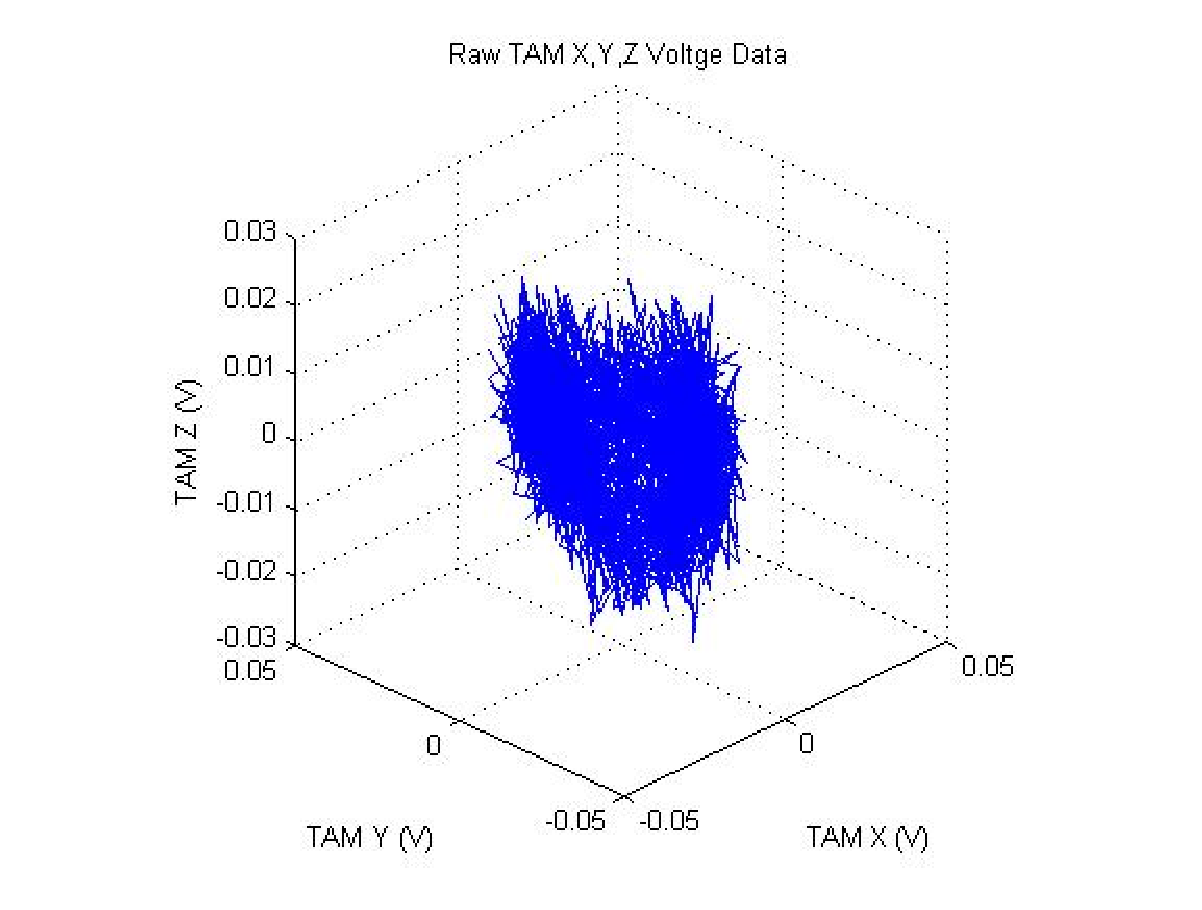
\psfig{file=figures/tam_raw.eps,height=4in}}
\caption{Raw TAM Voltages}
\label{fig:TAMRaw}
\end{figure}

Besides the slightly less dense center, the raw TAM measurements amount to a nebulous set of points with no clear pattern.  If the signal is strong enough, a consistent path should be present.  The evolution of data acquisition interpretation is presented here.  A basic 40 point moving average is attemped as a first pass analysis to verify that there is a defined signal in the data (Eq \ref{eqn:TAMMovingAvg}).  The moving average smoothed data is show in Figure \ref{fig:TAMMovingAverage}.  The good news being that a distinct an repeatable signal occurs as TableSat completes successive rotations.  The bad news is the irregular path that the magnetometer readings follow.

\begin{equation}
  x_i = \frac{1}{40} \sum^{39}_{j=0} x_{i-j}
  \label{eqn:TAMMovingAvg}
\end{equation}

\begin{figure}
  \begin{subfigure}[h!]{0.5\textwidth}
    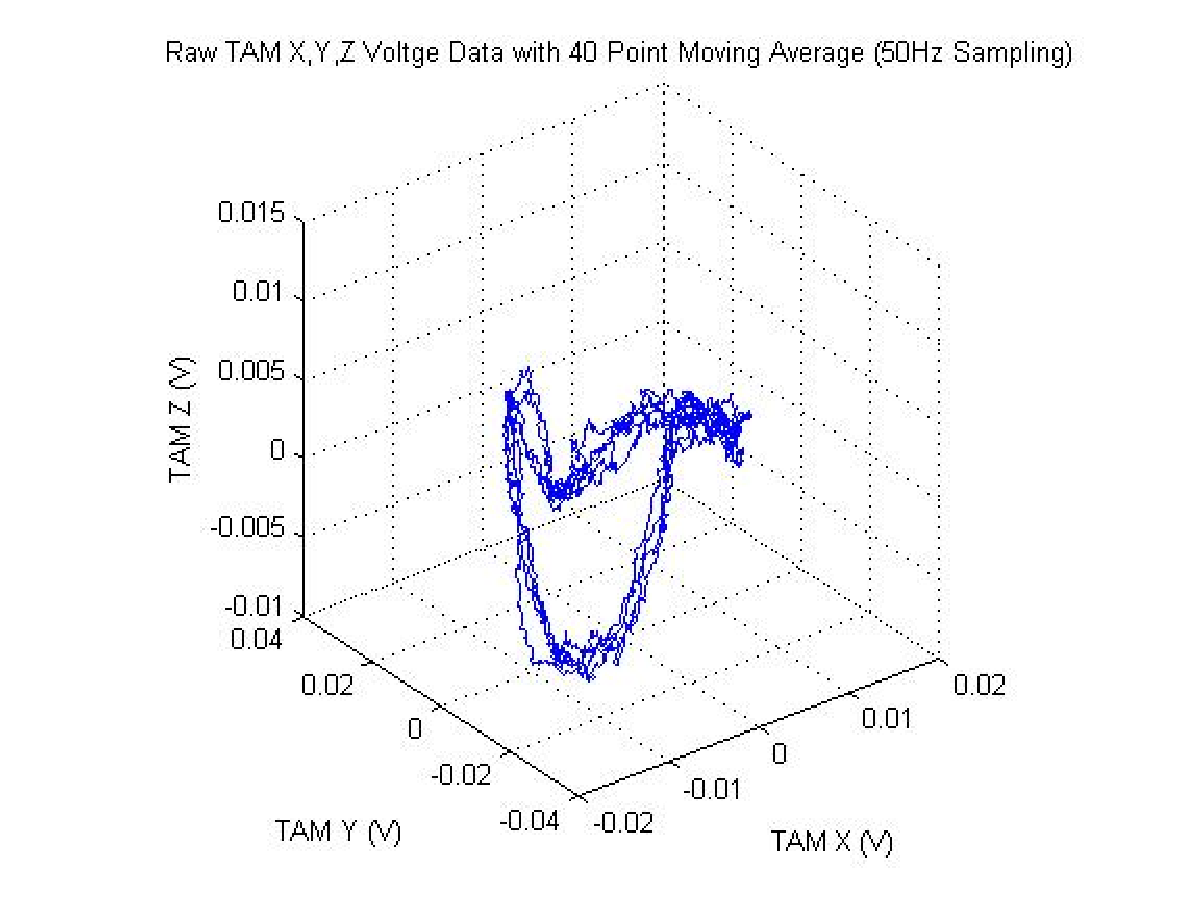
\includegraphics[width=\textwidth]{figures/tam_moving_average.eps}
    \caption{Raw TAM Voltages - Moving Average}
    \label{fig:TAMMovingAverage}
  \end{subfigure}
  ~
  \begin{subfigure}[h!]{0.5\textwidth}
    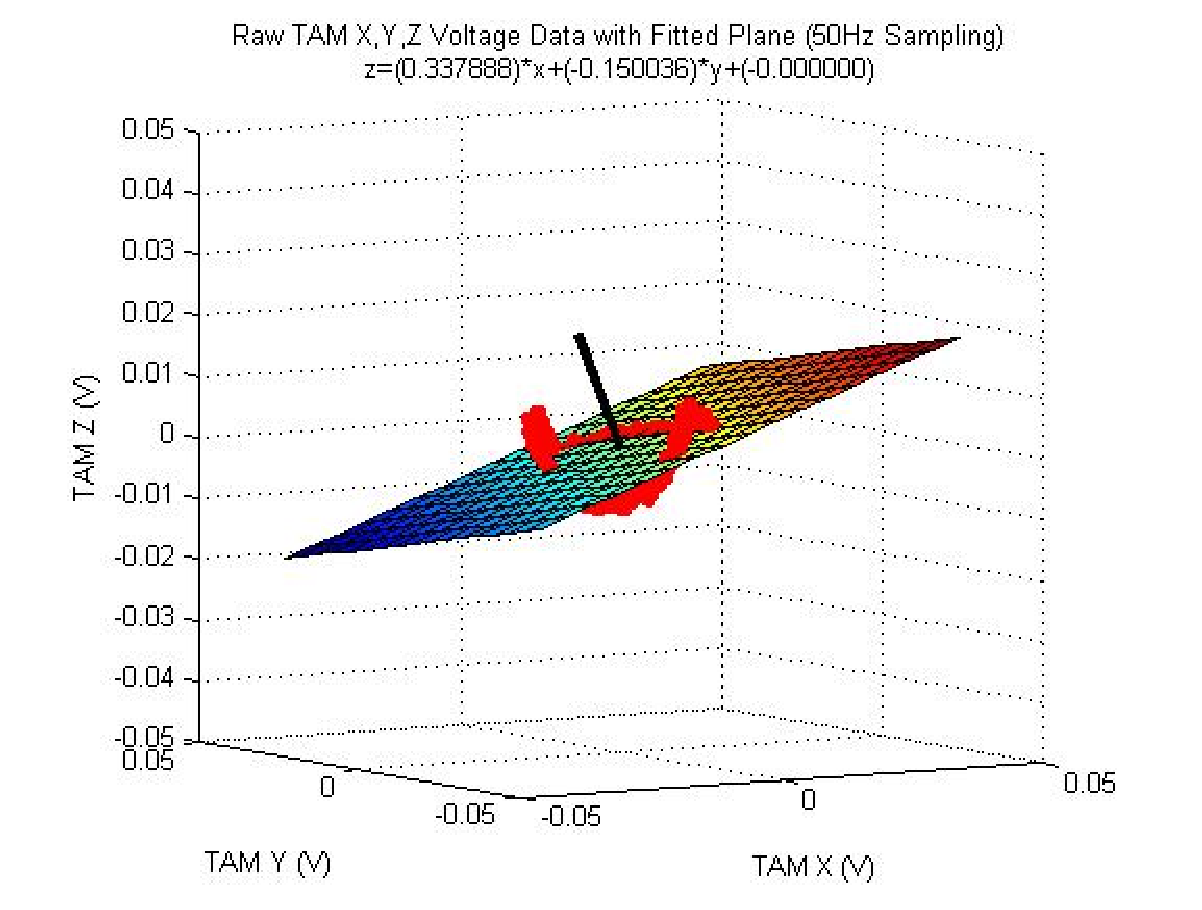
\includegraphics[width=\textwidth]{figures/tam_fitted_plane.eps}
    \caption{TAM Voltages with Fitted Plane}
    \label{fig:TAMFittedPlane}
  \end{subfigure}
  \caption{Determining Attitude from TAM}
  \label{fig:TAMSignal}
\end{figure}

Figure \ref{fig:TAMFittedPlane} shows the result of fitting a plane to the moving average smoothed TAM voltages.  The error in the fit between the smoothed TAM data points and the planar fit are too large to have much confidence in using this measure for nutation detection.

Following this analysis, the magnetic field surrounding the experimental setup is tested.  Moving a compass through the test space shows large swings in magnetic field lines despite the TableSat being placed on a wooden table in the middle of the ACL lab.  Subsequent sweeps of the lab locates a space with a relatively uniform magnetic field.  A uniform thrust is applied to the clockwise actuator and voltage readings are recorded as before.  Performing the moving average smoothing provides verification of the expected behavior of the magnetometer (Fig \ref{fig:TAMUniformField})

\begin{figure}[H]
  \centerline{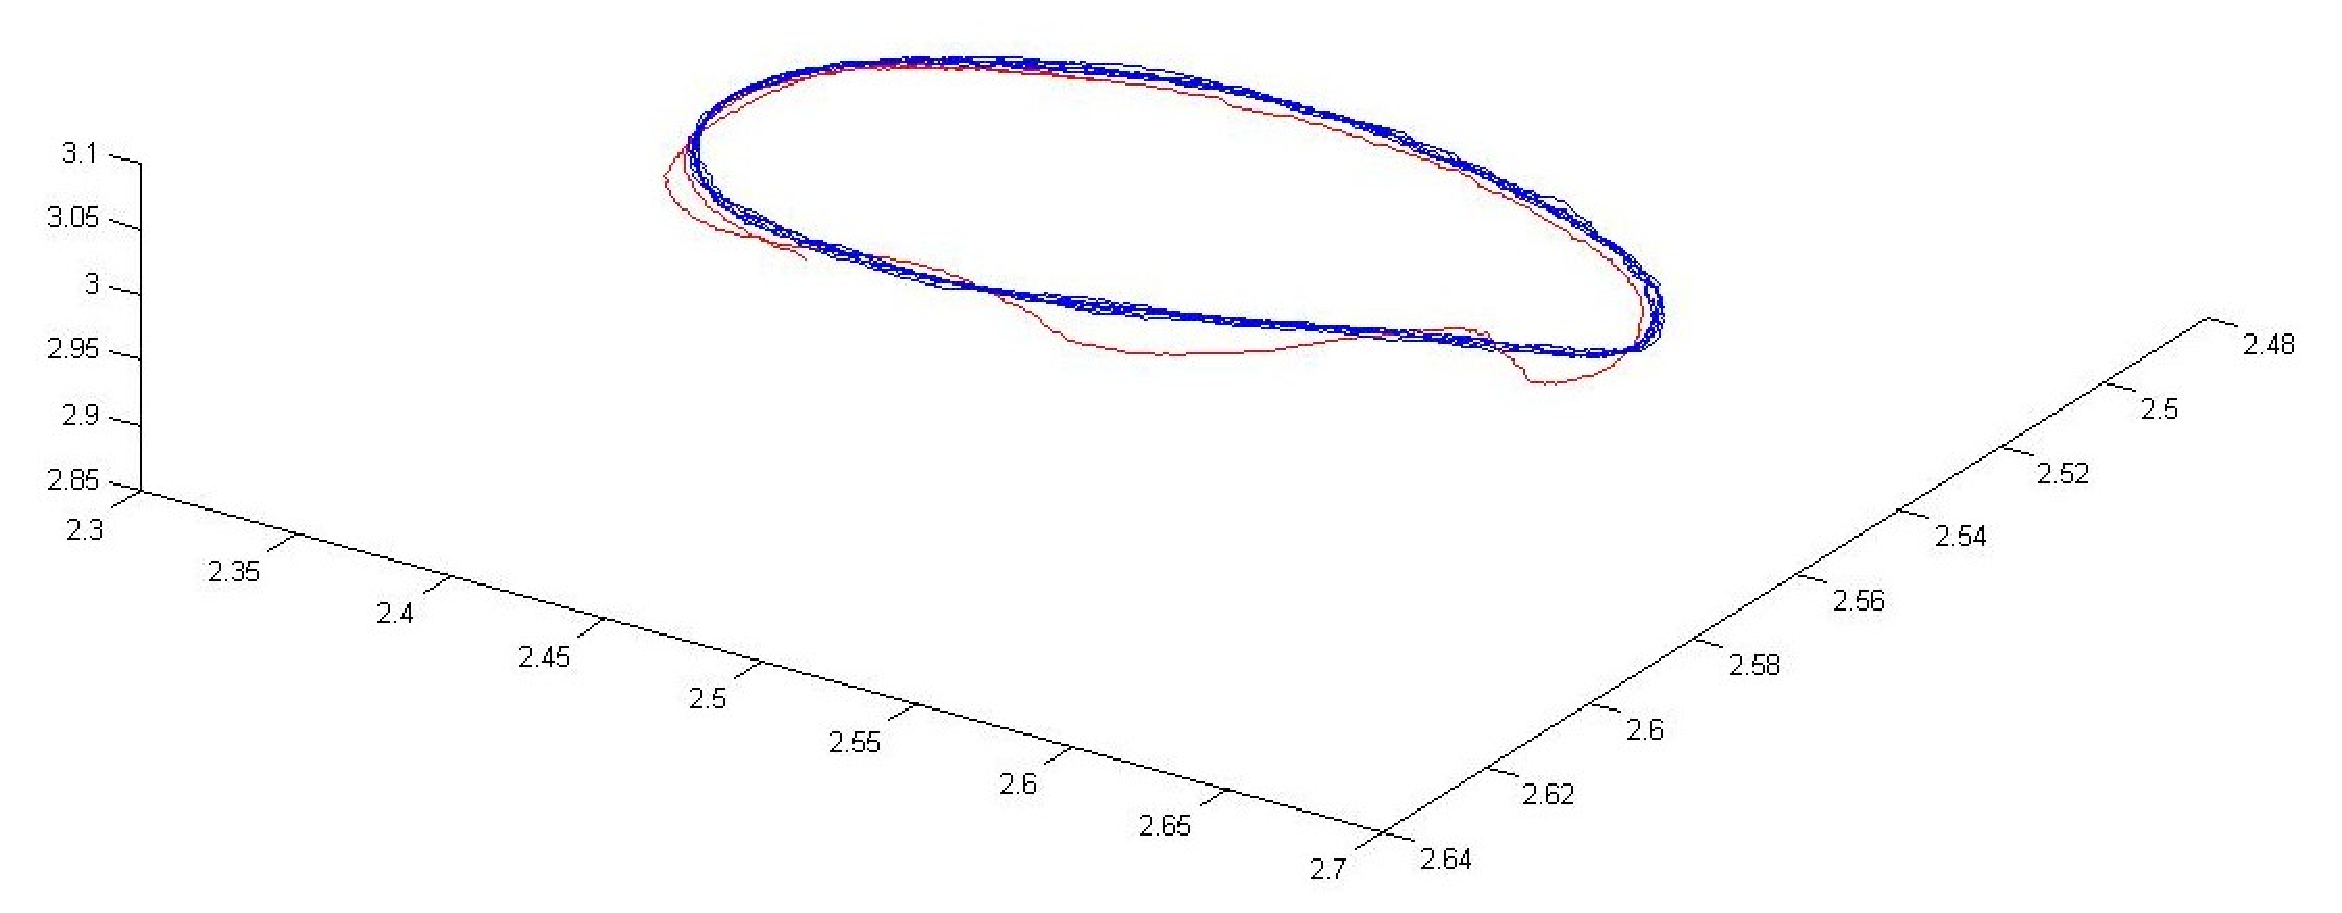
\psfig{file=figures/tam_uniform_field.eps,width=0.8\textwidth}}
  \caption{TAM measurements in a uniform field}
  \label{fig:TAMUniformField}
\end{figure}

Since the gyroscope and accelerometers are determined to be impractical for the observer-based controller and that the coarse sun sensors are only able to detect rotation about the z-axis, the three-axis magnetometer remains the only sensor with the capability to detect nutation required for the controller.

The baseline path established for TableSat in the absence of nutation (Figure \ref{fig:TAMUniformField}) should be able to be compared to readings during a ``live run'' of the system and any offsets used to quantify nutation.  The same process of rotating the TableSat under a constant thrust is repeated four more times.  Each time a 200g brass weight is placed on the TableSat's bus at each principle axis $+x, +y, -x, -y$ causing the TableSat to pivot about 14 degrees out of the spin plane approximately the extent of the TableSat's nutation range.  The TAM voltage readings for each test set are grouped by color and shown in Figure \ref{fig:TAMNutationVoltages}.  Although the paths intersect and measurements are not one-to-one correlation to the TableSat's orientation, there is at least a separation in paths.  Further study shows that while the TAM voltage outputs are duplicated between nutation paths, points that occupy the same space in the TAM measurement have different yaw measurements as measured by the coarse sun sensor.

\begin{figure}[H]
  \centerline{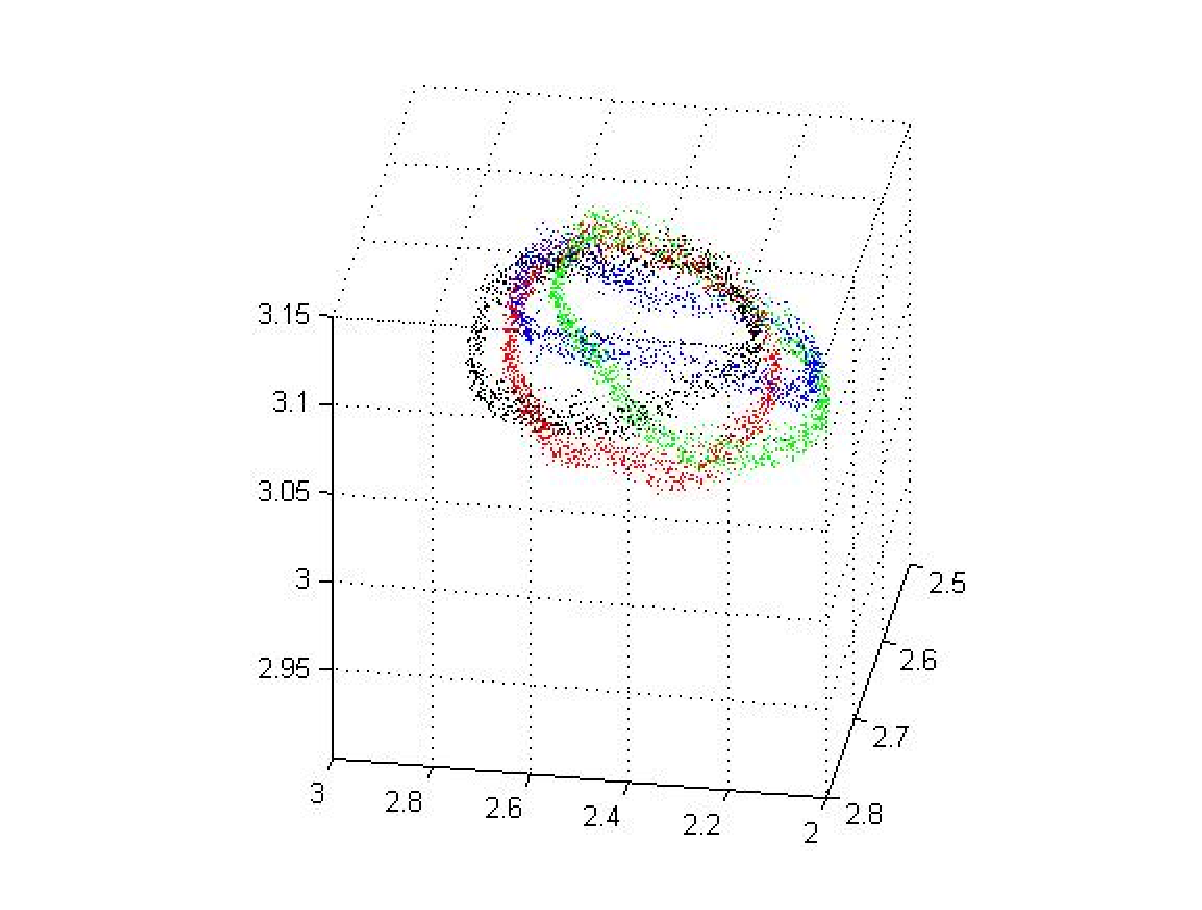
\psfig{file=figures/tam_distinct_tilts_with_good_field.eps,height=4in}}
  \caption{TAM nutation voltages}
  \label{fig:TAMNutationVoltages}
\end{figure}

\section{TableSat Attitude Measurement}
\label{subsec:StateMeasurement}

As covered in the sections above, the only sensors available for state measurement of TableSat IA for the observer-based controller are the coarse sun sensor and the three-axis magnetometer (TAM), both of which individually measure a portion of the system's attitude and leave the system's body rate unmeasured.

Combining the measurements of the coarse sun sensor and provide high confidence in the yaw measurement and rough estimates of roll and pitch nutation.  An algorithm is developed that is initialized with coarse sun sensor measurements and through Equation (\ref{eqn:CSSResultantForce}) produces a yaw measurement (i.e., rotation about the $z$-axis).  The TAM calibration data is synthesized to create a reference table of TAM readings at each of the five paths: level rotation and each of the four nutation shown in Figure \ref{fig:TAMNutationVoltages}.  This reference table along with the equation to determine yaw from the coarse sun sensor are combined through a method described in \label{subsec:CalculateTAMNutationReferenceData} to approximate the TableSat's attitude.  The general procedure is to scan the CSS output voltages and determine the yaw angle.  After which the table of TAM calibration voltages is referenced for the corresponding yaw and the five sets of path reading are returned.  From there the current TAM voltages are compared it $\Re^3$ with the five calibration points to determine which direction the TableSat is tilted.  For positions that do not directly correspond to a calibration point, the relative proximity to the nearest points are used to calculate a nutation axis between the two calibration nutation angles.
